% Ready-to-paste LaTeX figure environments for the CU-MOBO paper.
% Main figure (Fig.1) is the compiled vector PDF figures/main_figure.pdf (TikZ source: figures/main_figure.tex).
% Result figures live in ../results/*.png. Adjust \graphicspath or paths as needed.
% Requires: \usepackage{graphicx}  (and \usepackage{subcaption} only if you split panels).

% \graphicspath{{figures/}{../results/}}

\begin{figure*}[t]
  \centering
  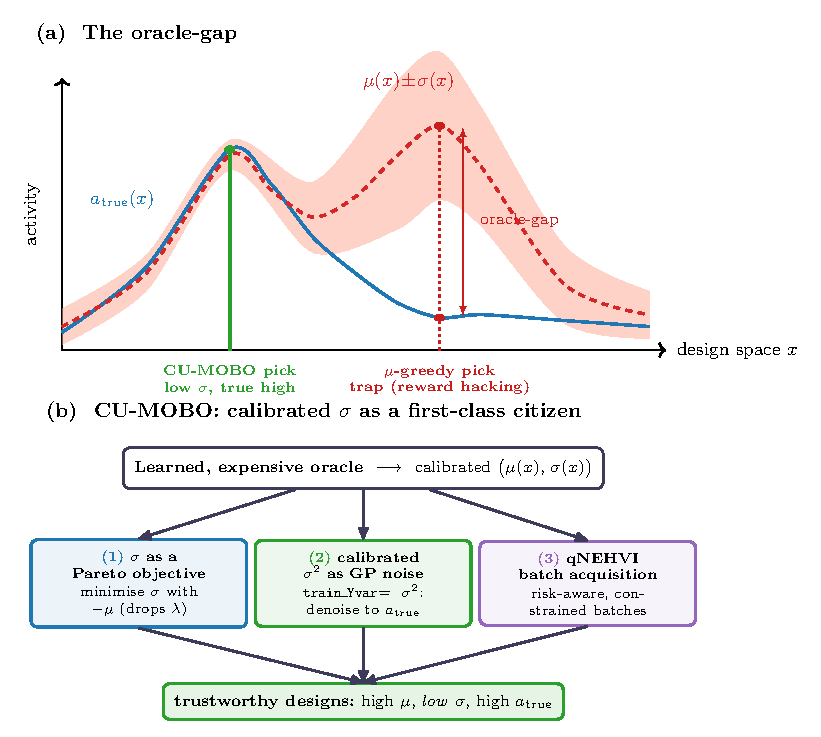
\includegraphics[width=\textwidth]{figures/main_figure.pdf}
  \caption{CU-MOBO at a glance. \textbf{(a)} The \emph{oracle-gap}: $\mu$-greedy optimisation
  chases a spurious $\mu$ peak where the calibrated $\sigma$ is large and the true activity
  $a_{\text{true}}$ is low (a trap / reward-hacking region), whereas reading $\sigma$ steers to
  the trustworthy optimum (high $\mu$, \textbf{low} $\sigma$, high $a_{\text{true}}$).
  \textbf{(b)} CU-MOBO turns the oracle's calibrated $\sigma$ into a first-class citizen through
  three mechanisms---$\sigma$ as a Pareto objective, calibrated $\sigma^2$ as heteroscedastic GP
  observation noise (\texttt{train\_Yvar}), and risk-aware qNEHVI batch acquisition---yielding
  trustworthy designs.}
  \label{fig:main}
\end{figure*}

\begin{figure}[t]
  \centering
  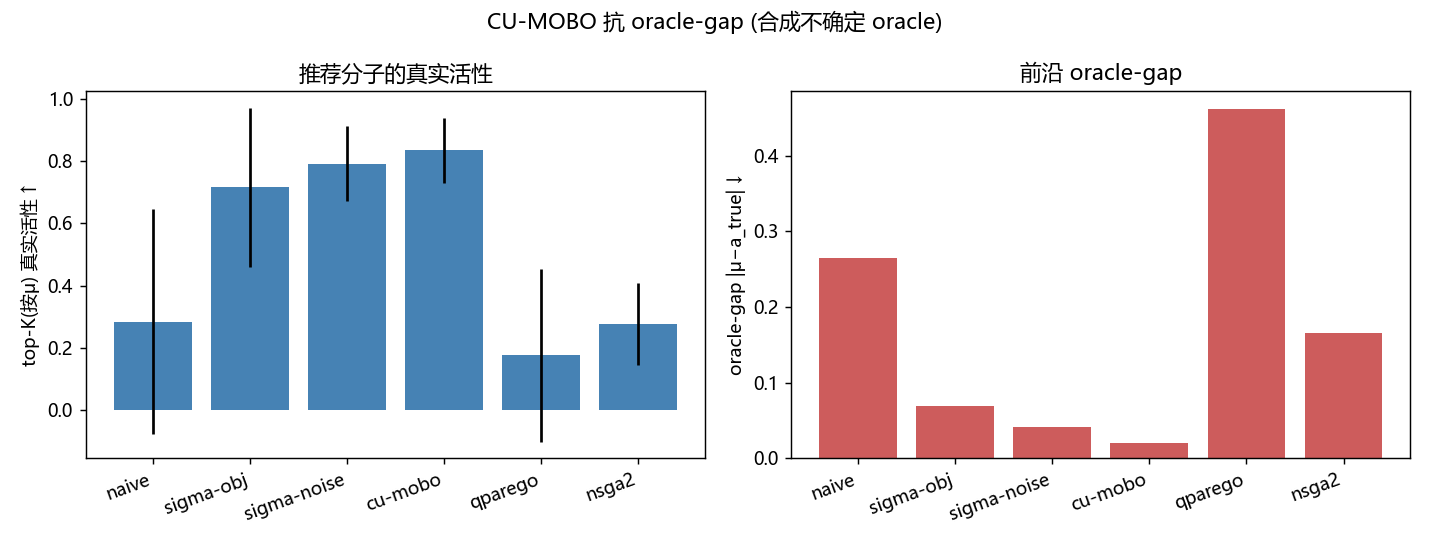
\includegraphics[width=\linewidth]{../results/oracle_gap.png}
  \caption{Controlled synthetic oracle-gap benchmark (5 seeds, hidden ground truth).
  \emph{Left:} true activity of the top-$K$ recommended designs ($\uparrow$)---CU-MOBO and its
  $\sigma$-ablations dominate the no-$\sigma$ baselines (naive, qParEGO, NSGA-II).
  \emph{Right:} front oracle-gap $|\mu-a_{\text{true}}|$ ($\downarrow$). The $2\times2$ ablation
  is monotone: each $\sigma$ mechanism helps and the two are complementary.}
  \label{fig:oraclegap}
\end{figure}

\begin{figure}[t]
  \centering
  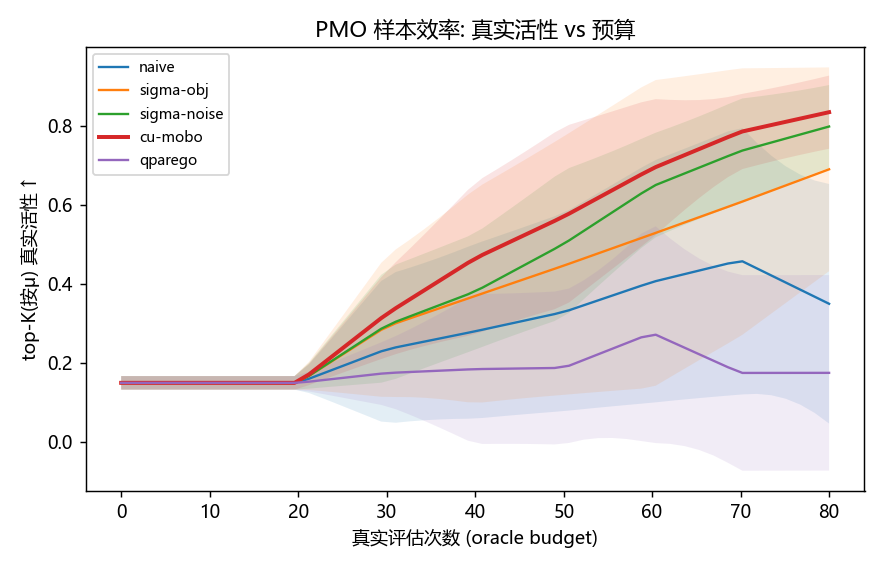
\includegraphics[width=\linewidth]{../results/oracle_gap_convergence.png}
  \caption{PMO sample efficiency: true activity of the top-$K$ (by $\mu$) designs vs
  real-evaluation budget (mean $\pm$ sd, 5 seeds). CU-MOBO reaches high \emph{true} activity
  soonest per expensive oracle call; the $\mu$-only baselines (naive, qParEGO) plateau low
  because they spend budget in oracle-gap regions.}
  \label{fig:pmo}
\end{figure}

\begin{figure}[t]
  \centering
  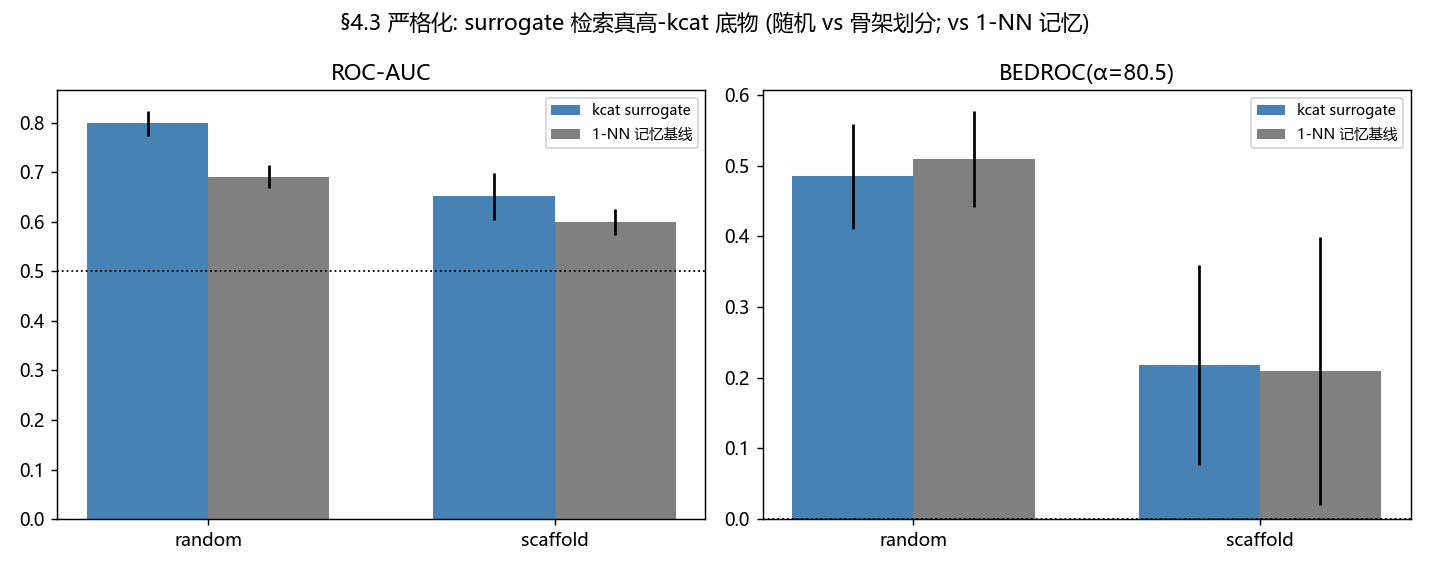
\includegraphics[width=\linewidth]{../results/retrospective_hardened.png}
  \caption{Hardened retrospective screening on real kcat labels. Enrichment Factor /
  BEDROC($\alpha{=}80.5$) / ROC-AUC of the leakage-controlled surrogate under random vs
  Bemis--Murcko \textbf{scaffold} splits, against a 1-NN memorization baseline, with bootstrap
  95\,\% CIs (5 seeds). The surrogate generalises to unseen scaffolds (AUC 0.65, CI excludes 0.5)
  and beats 1-NN; the random$\to$scaffold drop quantifies analogue bias.}
  \label{fig:retro}
\end{figure}

\begin{figure}[t]
  \centering
  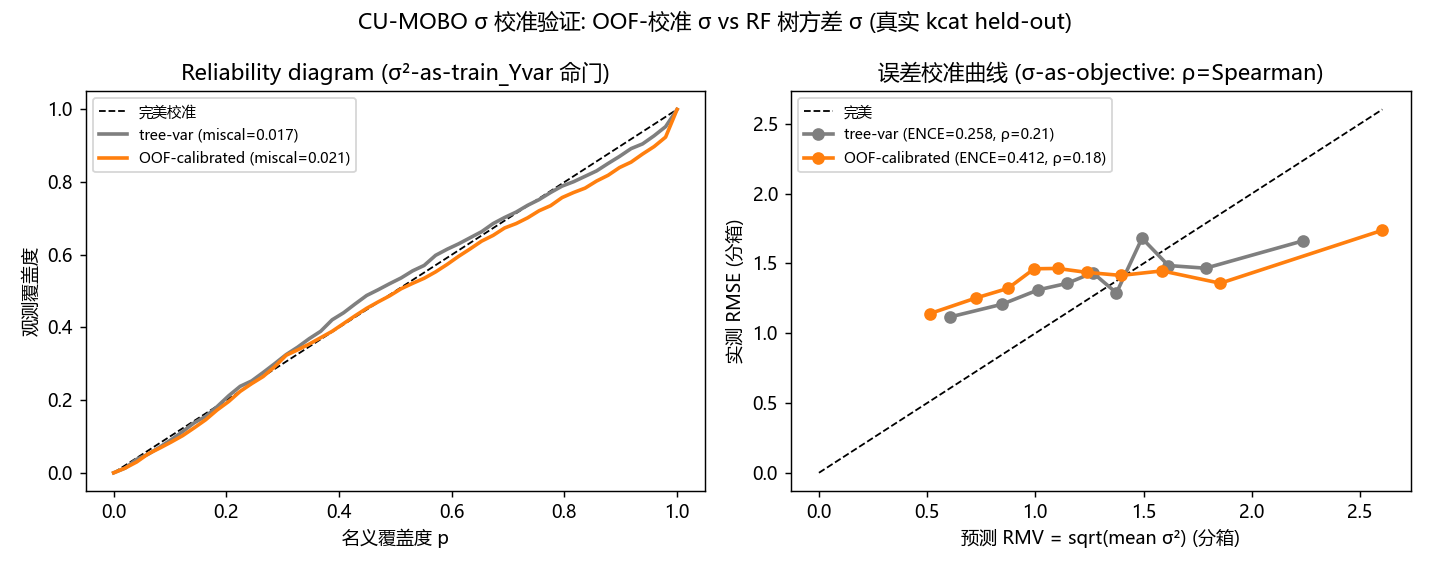
\includegraphics[width=\linewidth]{../results/calibration.png}
  \caption{$\sigma$-calibration audit on the real-kcat surrogate. Reliability diagram, ENCE and
  Spearman $\rho(\sigma,|\text{error}|)$ for tree-variance vs OOF-residual $\sigma$. Both are
  only weakly (though significantly) calibrated ($\rho\approx0.2$), and the OOF head does
  \emph{not} beat tree variance---obtaining calibrated $\sigma$ on a real noisy oracle is itself
  the bottleneck (motivating extension E2).}
  \label{fig:calib}
\end{figure}

\begin{figure}[t]
  \centering
  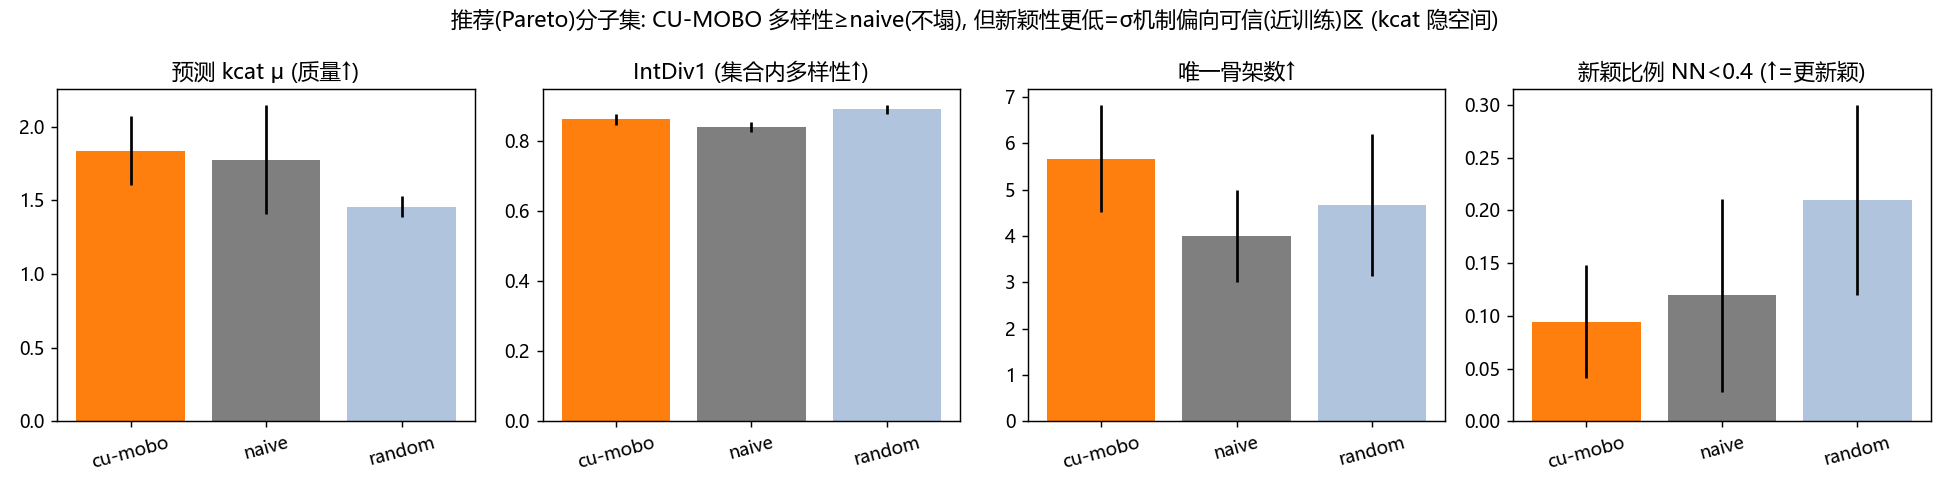
\includegraphics[width=\linewidth]{../results/diversity.png}
  \caption{Diversity and novelty of the recommended set (3 seeds): IntDiv$_1$, \#Circles,
  scaffold count and nearest-neighbour Tanimoto to the oracle's training set, for CU-MOBO vs
  $\mu$-greedy vs random. CU-MOBO does \emph{not} collapse diversity to resist the gap, but its
  recommendations are the least novel---the honest novelty$\leftrightarrow$reliability tradeoff
  of $\sigma$-aware search.}
  \label{fig:diversity}
\end{figure}

\begin{figure}[t]
  \centering
  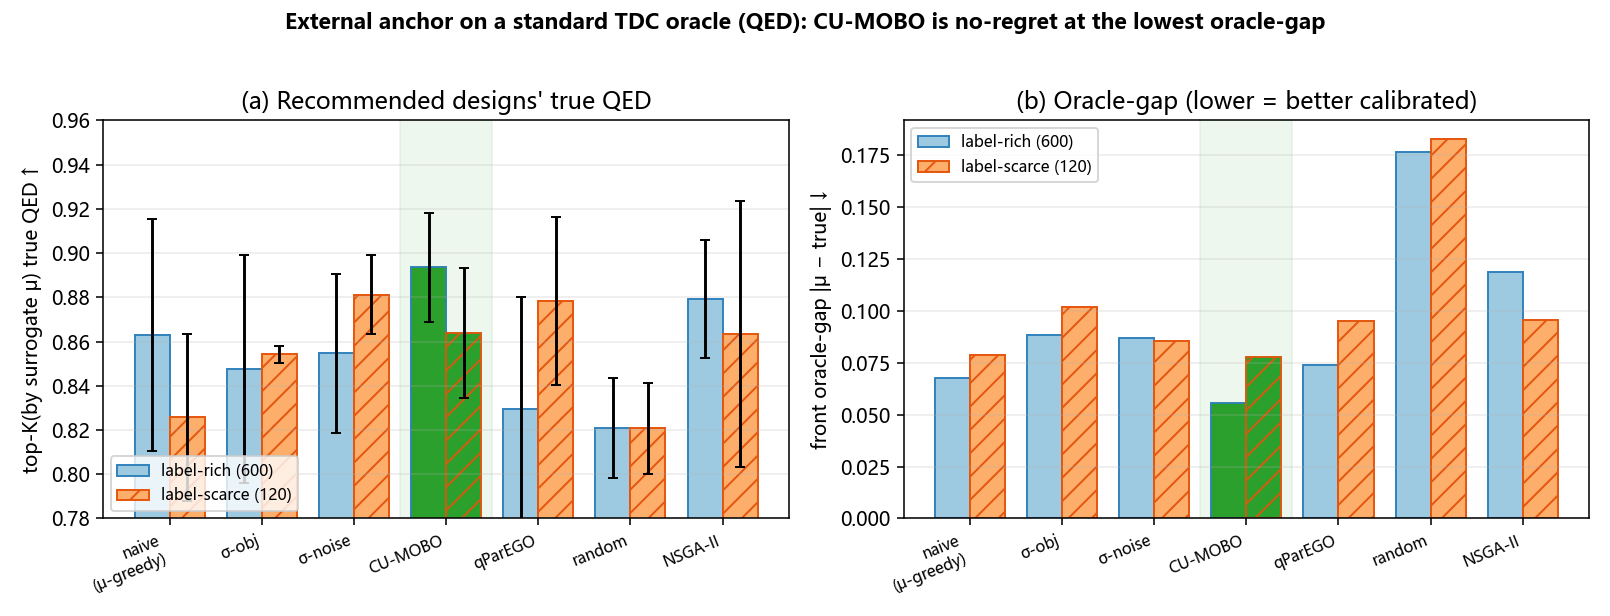
\includegraphics[width=\linewidth]{../results/tdc_anchor.png}
  \caption{External anchor on a community-standard TDC oracle (QED), 3 seeds, at two surrogate
  label budgets (rich 600 / scarce 120). \textbf{(a)} True QED of the top-$K$ designs;
  \textbf{(b)} front oracle-gap. CU-MOBO is \textbf{no-regret}---matching or edging $\mu$-greedy
  on activity---at the \textbf{lowest oracle-gap} in both budgets, on a third-party scorer with
  no circular logic.}
  \label{fig:tdc}
\end{figure}

\begin{figure}[t]
  \centering
  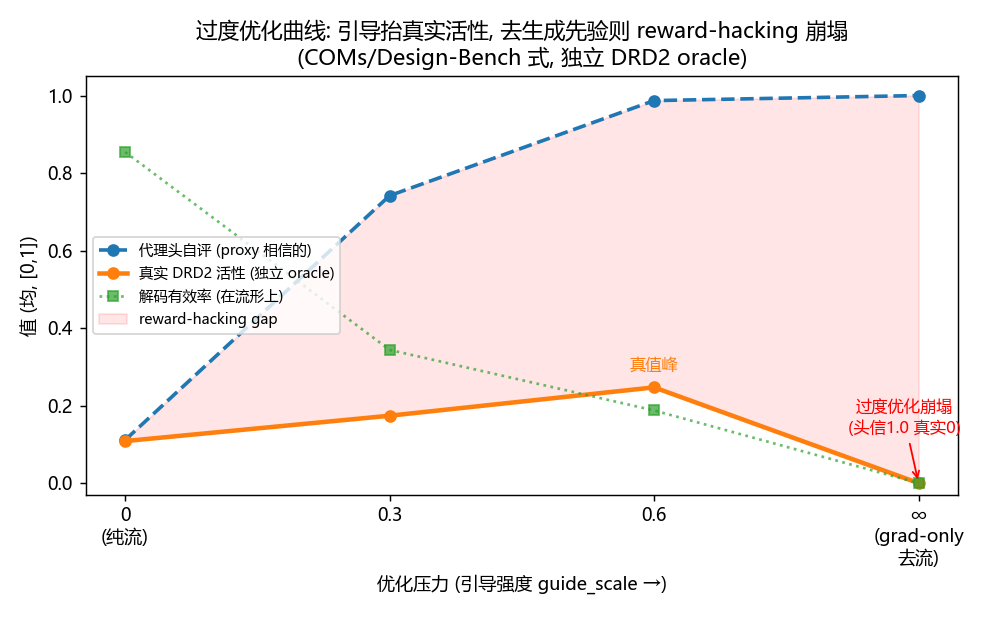
\includegraphics[width=\linewidth]{../results/overoptimization.png}
  \caption{E4 over-optimization (COMs-style) curve. As the flow-guidance strength $s$ increases
  ($0\to0.3\to0.6\to\infty$ = gradient-ascent only), the proxy head's self-belief rises
  \emph{monotonically} while true activity (scored by an \emph{independent} oracle) peaks at
  $s{=}0.6$ then \textbf{collapses} once the flow prior is removed---the reward-hacking signature
  reappearing inside the generator; the flow prior is the on-manifold regulariser.}
  \label{fig:overopt}
\end{figure}
